\section{Bootstrap}
Bootstrap anvendes ofte til at undersøge statistiske egenskaber af komplekse estimatorer.
For at motivere dets anvendelses, antager vi, at have fået et estimat \(\hat{\beta} \del{\hat{\lambda}_{\text{CV}}}\) for et lasso problem udfra følgende procedure, kaldet krydsvalidering:
%
\begin{enumerate}
\item Fit en lasso sti til \(\del{\X, \y}\) over en række værdier af \(\lambda\), dvs \(\Lambda = \cbr{\lambda_\ell}_{\ell=1}^L\).
\item Opdel tilfældigt det fulde datasæt ligeligt i \(K\) grupper. Typisk vælges \(K\) til at være lig 5 eller 10.
\item Lad én af disse grupper være testmængden, og betegn de resterende \(K-1\) grupper som træningsmængden. 
Anvend lasso på træningsmængden over \(\Lambda\), hver af disse fittede modeller anvendes til at prædiktere responserne i testmængden, hvilket giver gennemsnitlige-kvadrerede prædiktions fejl for hver værdi af \(\lambda\). 
\item Dette gøres for hver gruppe \(K\). Hermed fås \(K\) estimater af prædiktions fejlen over \(\Lambda\). 
Vi tager gennemsnittet af disse K estimater af prædiktions fejlen for hver værdi af \(\lambda\), hvorved vi finder krydsvaliderings fejl kurven.
\item Find værdien \(\hat{\lambda}_{\text{CV}}\) som minimerer denne kurve, og returnerer da koefficientvektoren fra det originale fit i step (1) for denne værdi af $\lambda$
\end{enumerate}
\texttt{R}-pakken \texttt{glmnet} som anvendes til at udføre krydsvalidering har by default \(K=10\).
%
\begin{figure}[H]
\centering
 \scalebox{0.5}{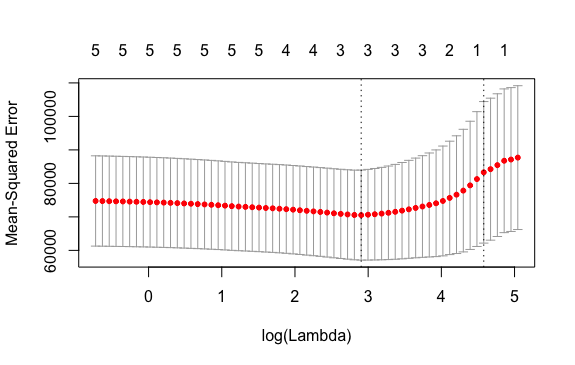
\includegraphics{fig/CV_error_crime.png}}
\caption{Krydsvaliderings estimat af den gennemsnitlige kvadrerede prædiktions fejl, som en funktion af \(\log \del{\lambda}\).}
\label{fig:CV_error_crime}
\end{figure}
%
Figur \ref{fig:CV_error_crime} viser krydsvaliderings fejl kurven for crime data hvor \(K=10\). FORKLARING
Dette er den mindste værdi af \(\lambda\) som giver en CV fejl indenfor en standard fejl af dens minimum.
Antallet af ikke-nul koefficienter i hver model vises i toppen.
Dermed har modellen som minimerer CV fejlen tre prædiktorer, mens 

Bootstrap anvendes da til at vurdere fordelingen af \(\hat{\beta} \del{\hat{\lambda}_{\text{CV}}}\) -- ikke-parametrisk og parametrisk??
boxplot og bootstrap plot

 